As mentioned in \cref{sec:arkani-hamed-dimop} in the \gls{add} model, the
fundamental scale of the gravitational interaction, $\md$, is brought close to
the electroweak scale. At these energies, due to the large center of mass energy
available at \gls{lhc}, the predictions of the \gls{eft} become unreliable. For
this reason two different sets of limits have been calculated, one where the
full cross section is used and the other where it is weighted down by a factor
$\md^4/\hat{s}^2$ for events in which $\hat{s} > \md^2$, where $\hat{s}$ is the
center of mass energy of the initial partons involved in
\cref{fig:add_feynman}~\cite{LEDWeightFactor}. The general idea of weighting the
events is therefore introduced. It consists in re-evaluating the limit on $\md$
in a conservative way, by prescribing that all events with $\hat{s}$ exceeding
the validity limit should only weakly contribute to the limit on $\md$.

The selection of the missing transverse energy changes the $\hat{s}$
distribution as discussed below. Therefore the validity of the \gls{eft} needs
to be evaluated in each $\met$ bin used in the analysis. As an illustration of
the problem \cref{fig:shat} shows the $\hat{s}$ distribution for \gls{add}
events surviving a signal region selection with $250 < \met < 300$~GeV and
$700 < \met < 800$~GeV for the n = 3 and 6 extra dimensions models. The straight
line indicates the excluded $\md$ value before any weighting of the events. This
figure shows that a fraction of the selected events in the signal regions have a
value of $\hat{s}$ that exceeds the limit of validity of the effective field
theory. \cref{fig:shat} shows that the bulk of the $\hat{s}$ distribution moves
towards higher energy values both in the case when the number of extra
dimensions and the $\met$ are increased. The first dependence is understood
considering the growth of the graviton mass with the number of extra dimensions
showed in \cref{fig:graviton_mass}: the production of gravitons with higher mass
requires higher $\hat{s}$ of the initial partons. A similar argument holds when
the $\met$ selection is increased, higher values of missing energy imply the
production of higher momentum gravitons. As shown in \cref{fig:shat}, only a
small fraction of events is beyond the \gls{eft} validity limit. The visible
event yields are recomputed in each $\met$ bin (as defined in
\cref{sec:event-selection-1}) and for each $n$ and, as hinted by
\cref{fig:shat}, the effect of the re-weighting is negligible.
\begin{figure}[!htb]
  \centering
  \begin{subfigure}{.48\linewidth}
    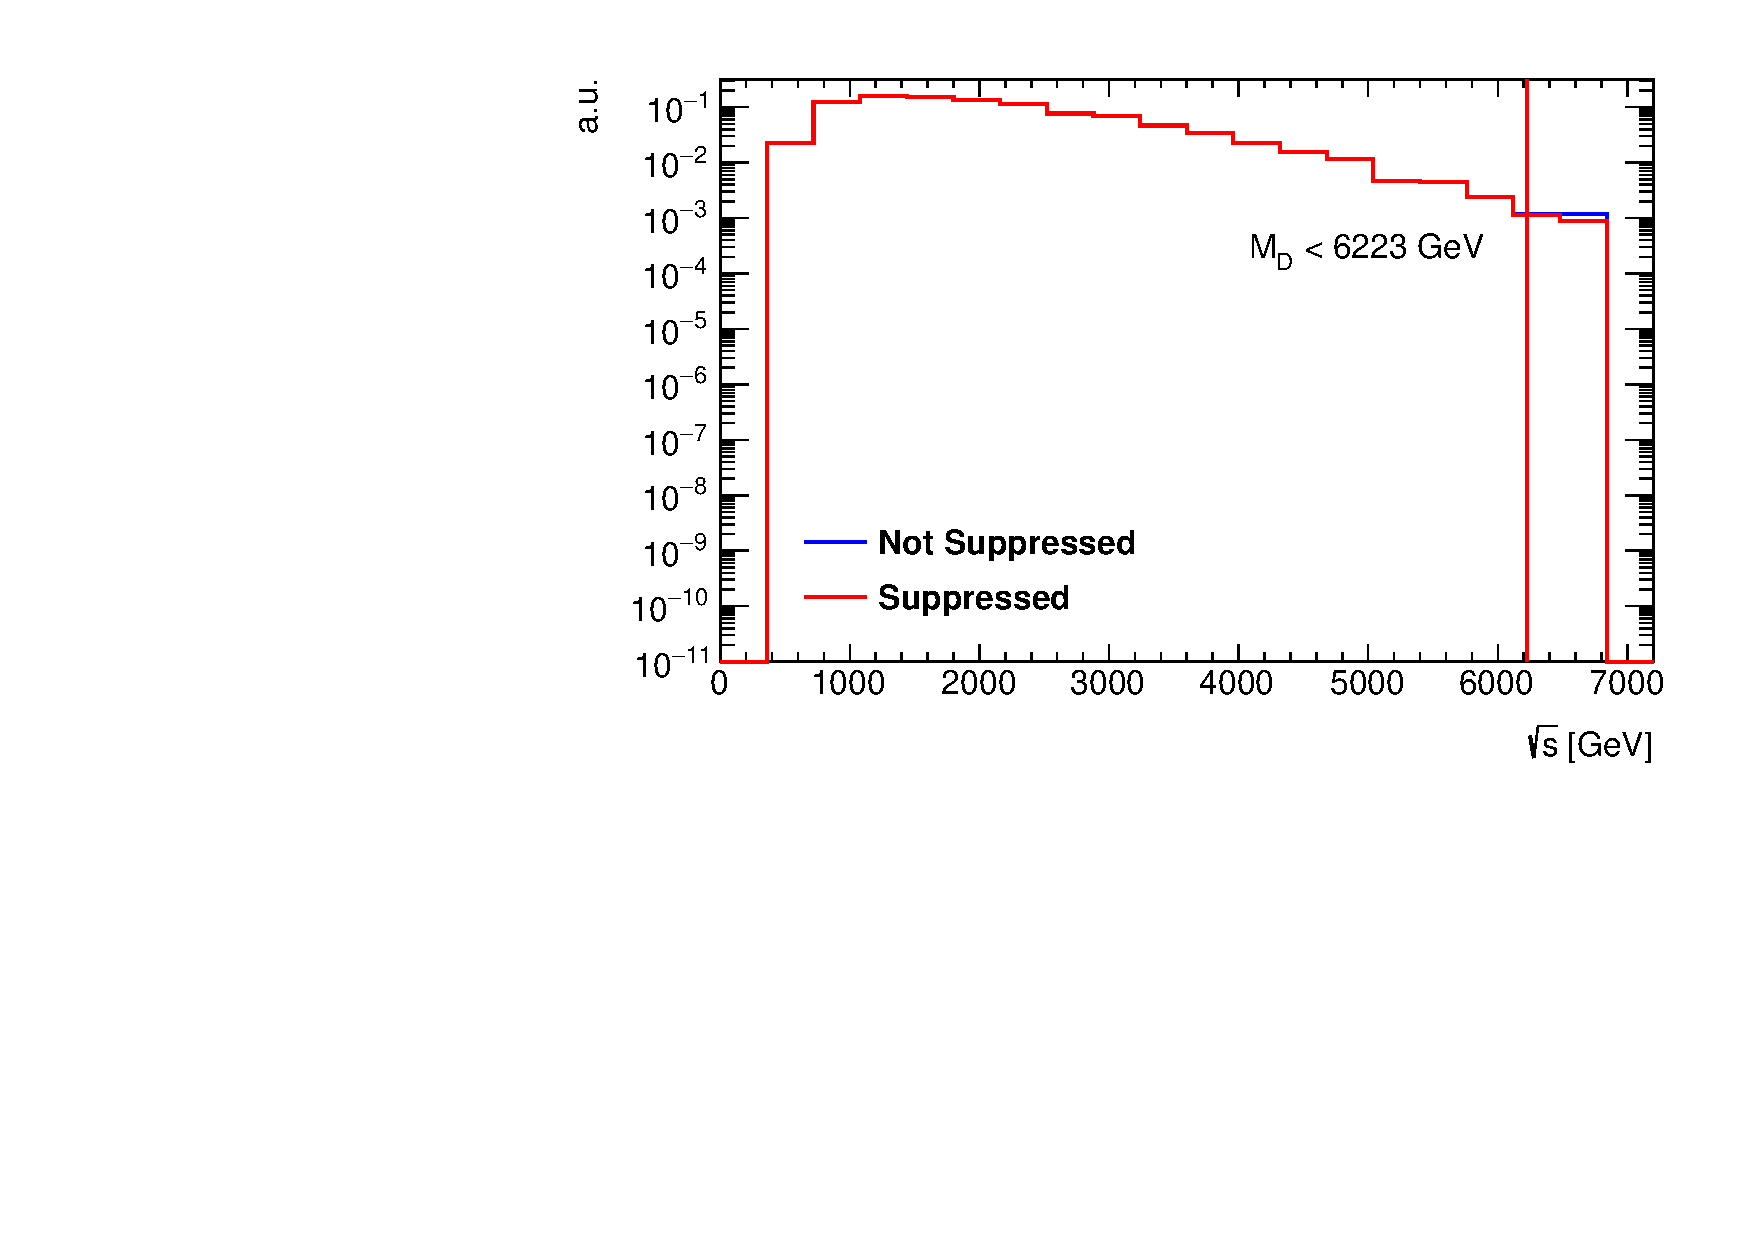
\includegraphics[width=\linewidth]{plot_nD3_SR250}
    \caption{ADD n = 3 for the low $\met$ region.}
    \label{fig:shat_n3_250}
  \end{subfigure}
  \begin{subfigure}{.48\linewidth}
    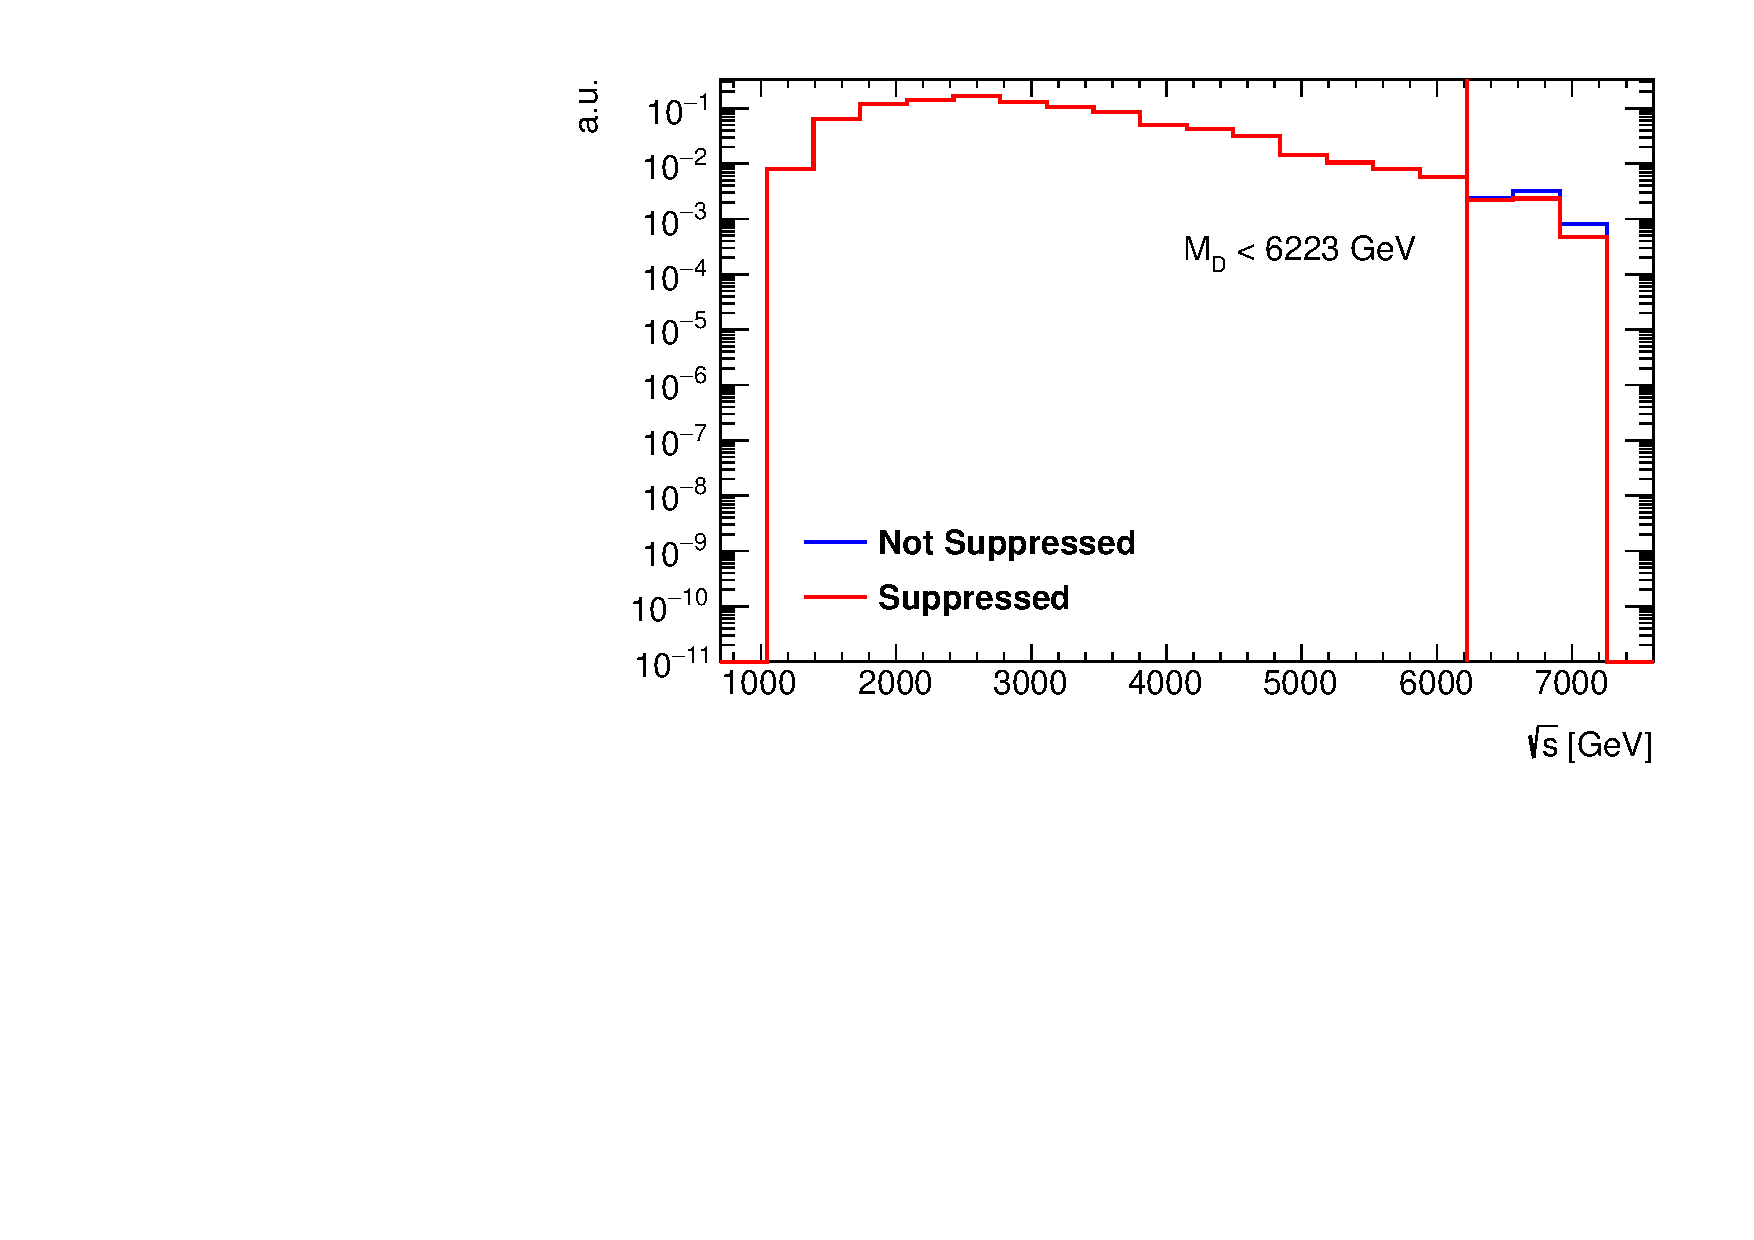
\includegraphics[width=\linewidth]{plot_nD3_SR700}
    \caption{ADD n = 3 for the high $\met$ region.}
    \label{fig:shat_n3_700}
  \end{subfigure}
  \begin{subfigure}{.48\linewidth}
    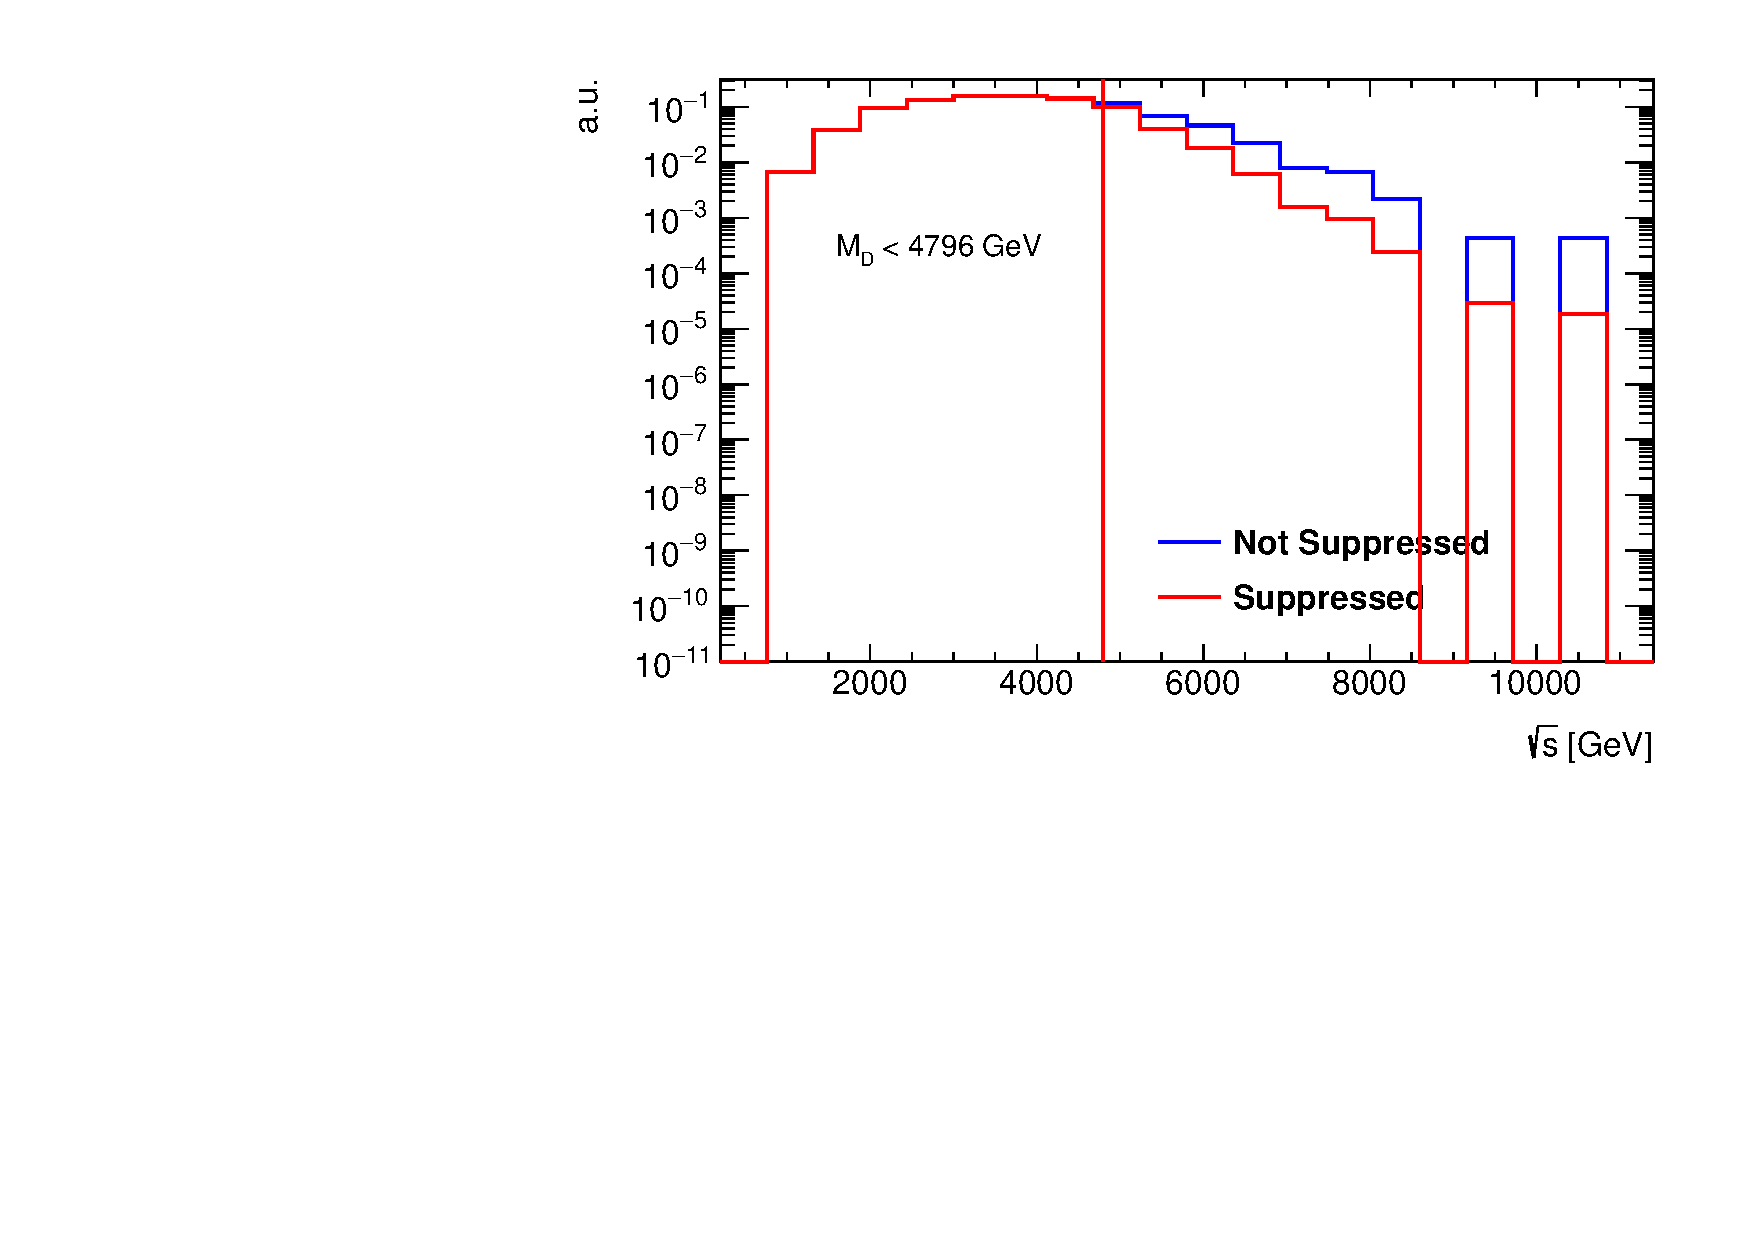
\includegraphics[width=\linewidth]{plot_nD6_SR250}
    \caption{ADD n = 6 for the low $\met$ region.}
    \label{fig:shat_n6_250}
  \end{subfigure}
  \begin{subfigure}{.48\linewidth}
    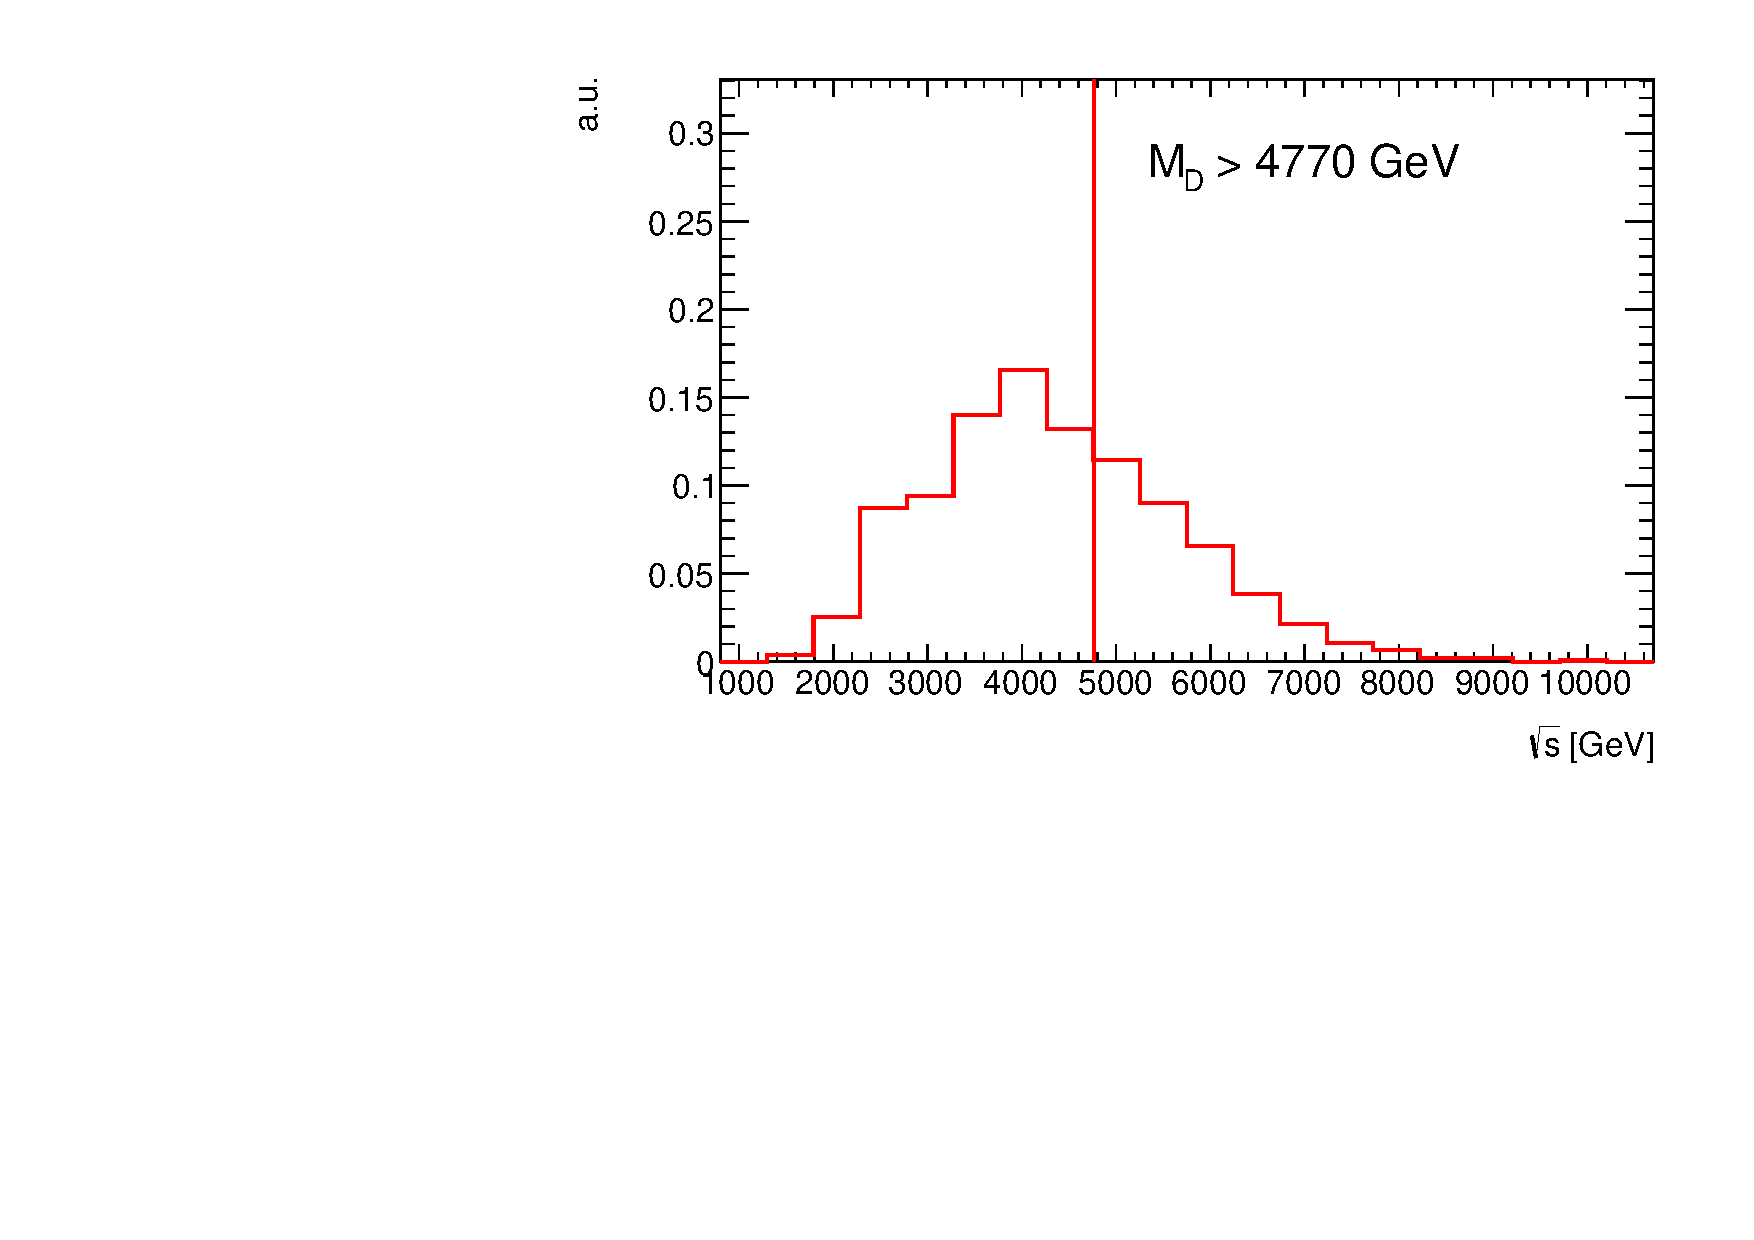
\includegraphics[width=\linewidth]{plot_nD6_SR700}
    \caption{ADD n = 6 for the high $\met$ region.}
    \label{fig:shat_n6_700}
  \end{subfigure}
  \caption{Generated $\hat{s}$ distribution with (blue) and without (red)
    weighting of the events for which $\hat{s} > \md^2$ for the signal regions
    where $250 < \met < 300$~GeV and $700 < \met < 800$~GeV for the ADD n = 3
    and 6 models for the 13~TeV \textsc{pythia8} Monte Carlo samples. A vertical
    line indicating the value of the excluded value of $\md$ is also reported in
    the figure.}
  \label{fig:shat}
\end{figure}
\begin{figure}[!htb]
  \centering
  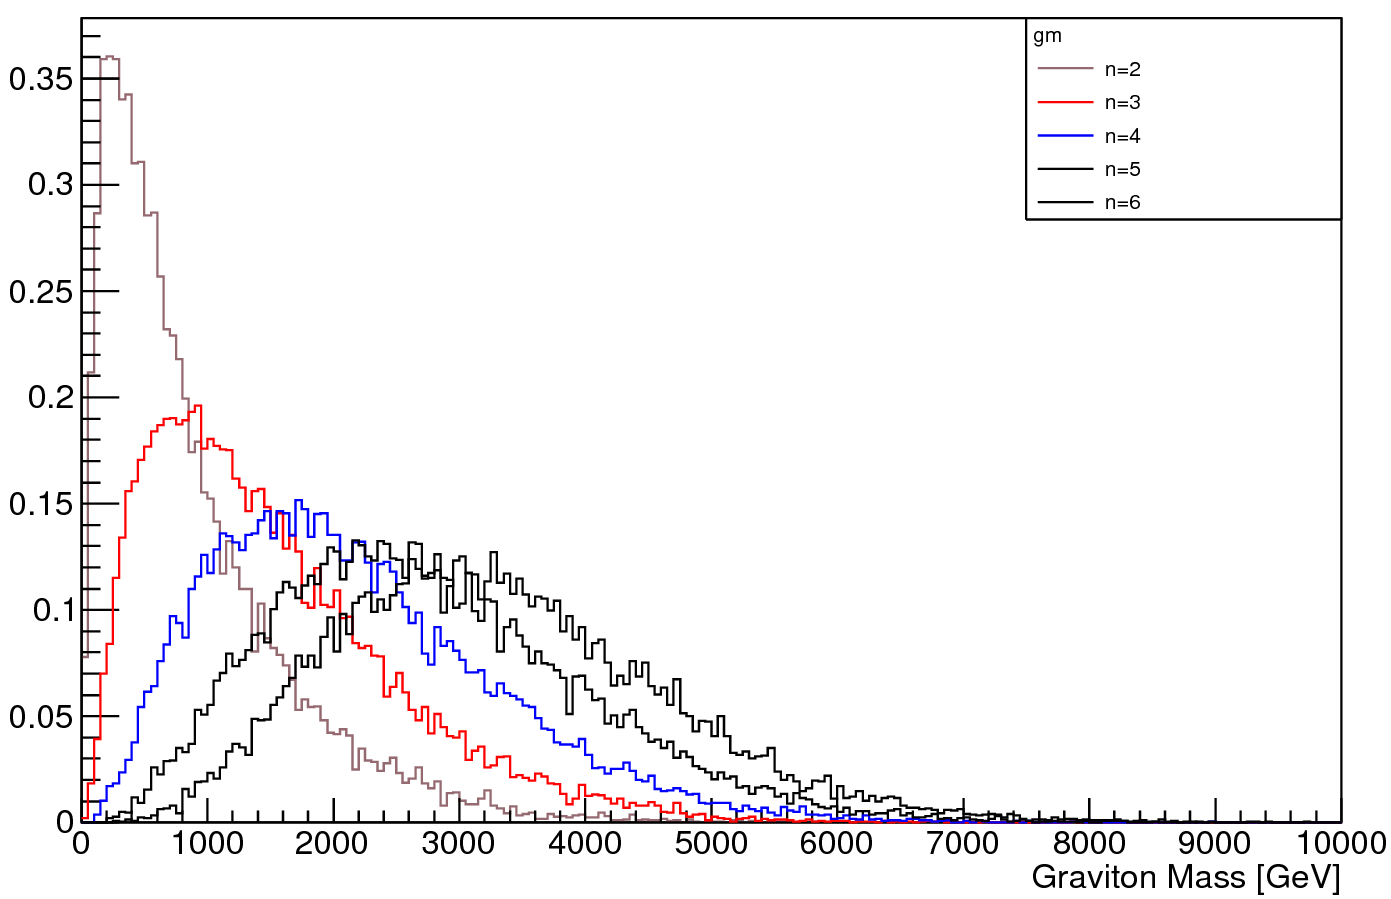
\includegraphics[width=.9\linewidth]{graviton_mass}
  \caption{Simulated heavy graviton masses for 2 to 6 extra dimensions in
    \gls{add} models computed with \textsc{pythia8} using the NNPDF23LO
    \gls{pdf} set and the A14 tunes~\cite{OllePhDThesis}.}
  \label{fig:graviton_mass}
\end{figure}

\cref{fig:vis_sigma_trunc} shows the visible cross section (see
\cref{sec:model-indep-limits}) as a function of the fundamental Planck scale
$\md$ in the $250 < \met < 300$~GeV and $700 < \met < 800$~GeV regions for the
ADD n = 3, 6 models. The solid line is the visible cross section when
considering the entire $\hat{s}$ range, while in the dashed line a
$\md^4/\hat{s}^2$ weighting factor is applied for events where
$\hat{s} > \md^2$. It can be seen that for $\md = 0$ all events would get
weighted down since $\hat{s} > \md^2 = 0$. The black square is the nominal $\md$
value of the generated sample listed in \cref{tab:sigma_md_ref}. The ratio of
the dashed red curve over the blue is used to scale down the exclusion limits in
each bin of $\met$ in order to take into account the effect of the validity of
the \gls{eft}. This effect is however smaller than the uncertainties on the
exclusions and is thus neglected. The $\hat{s}$ distribution is different for
each $\met$ bin which therefore receives a different suppression. The lowest
$\met$ bins are suppressed the least.
\begin{figure}[!htb]
  \centering
  \begin{subfigure}{.48\linewidth}
    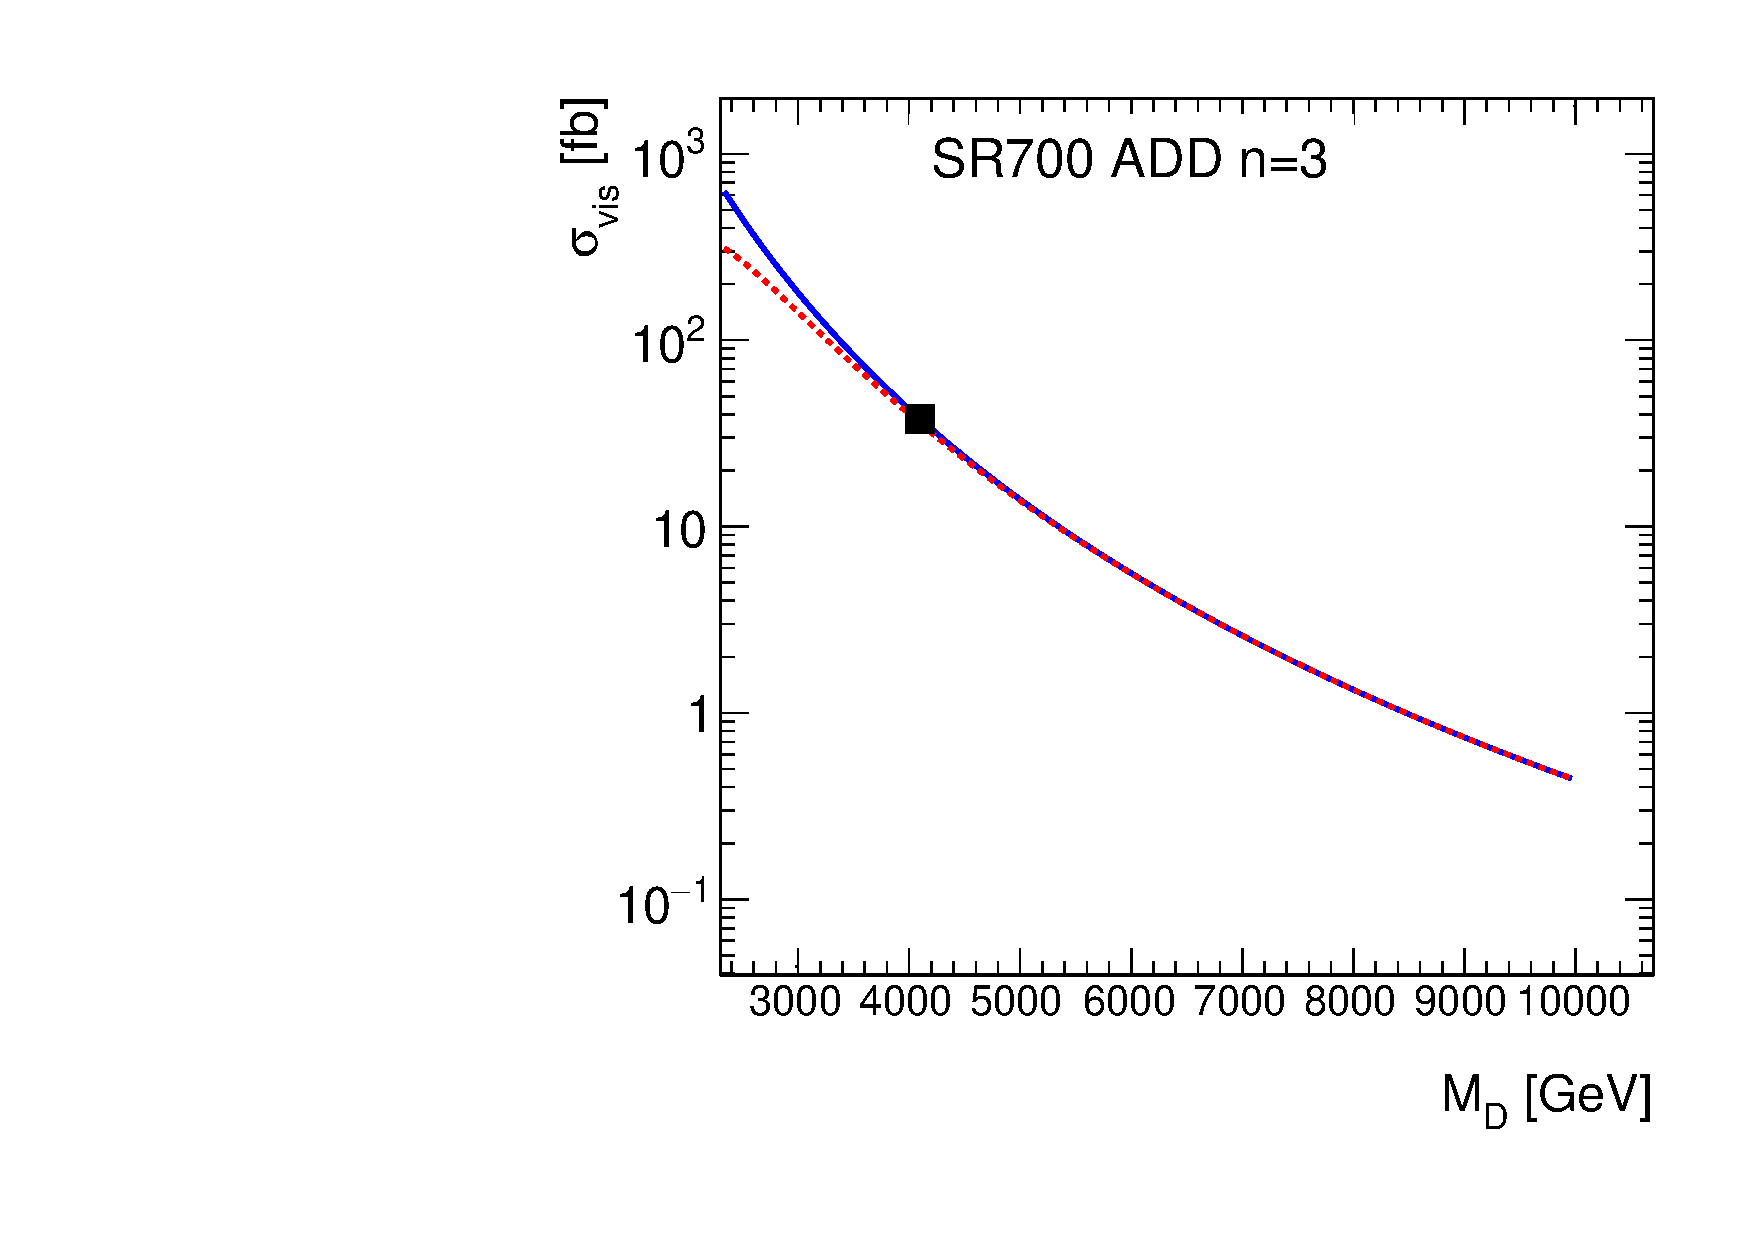
\includegraphics[width=\linewidth]{plot_sigma_visible_nD3_SR700}
    \caption{}
    \label{fig:sigma_vis_n3}
  \end{subfigure}
  \begin{subfigure}{.48\linewidth}
    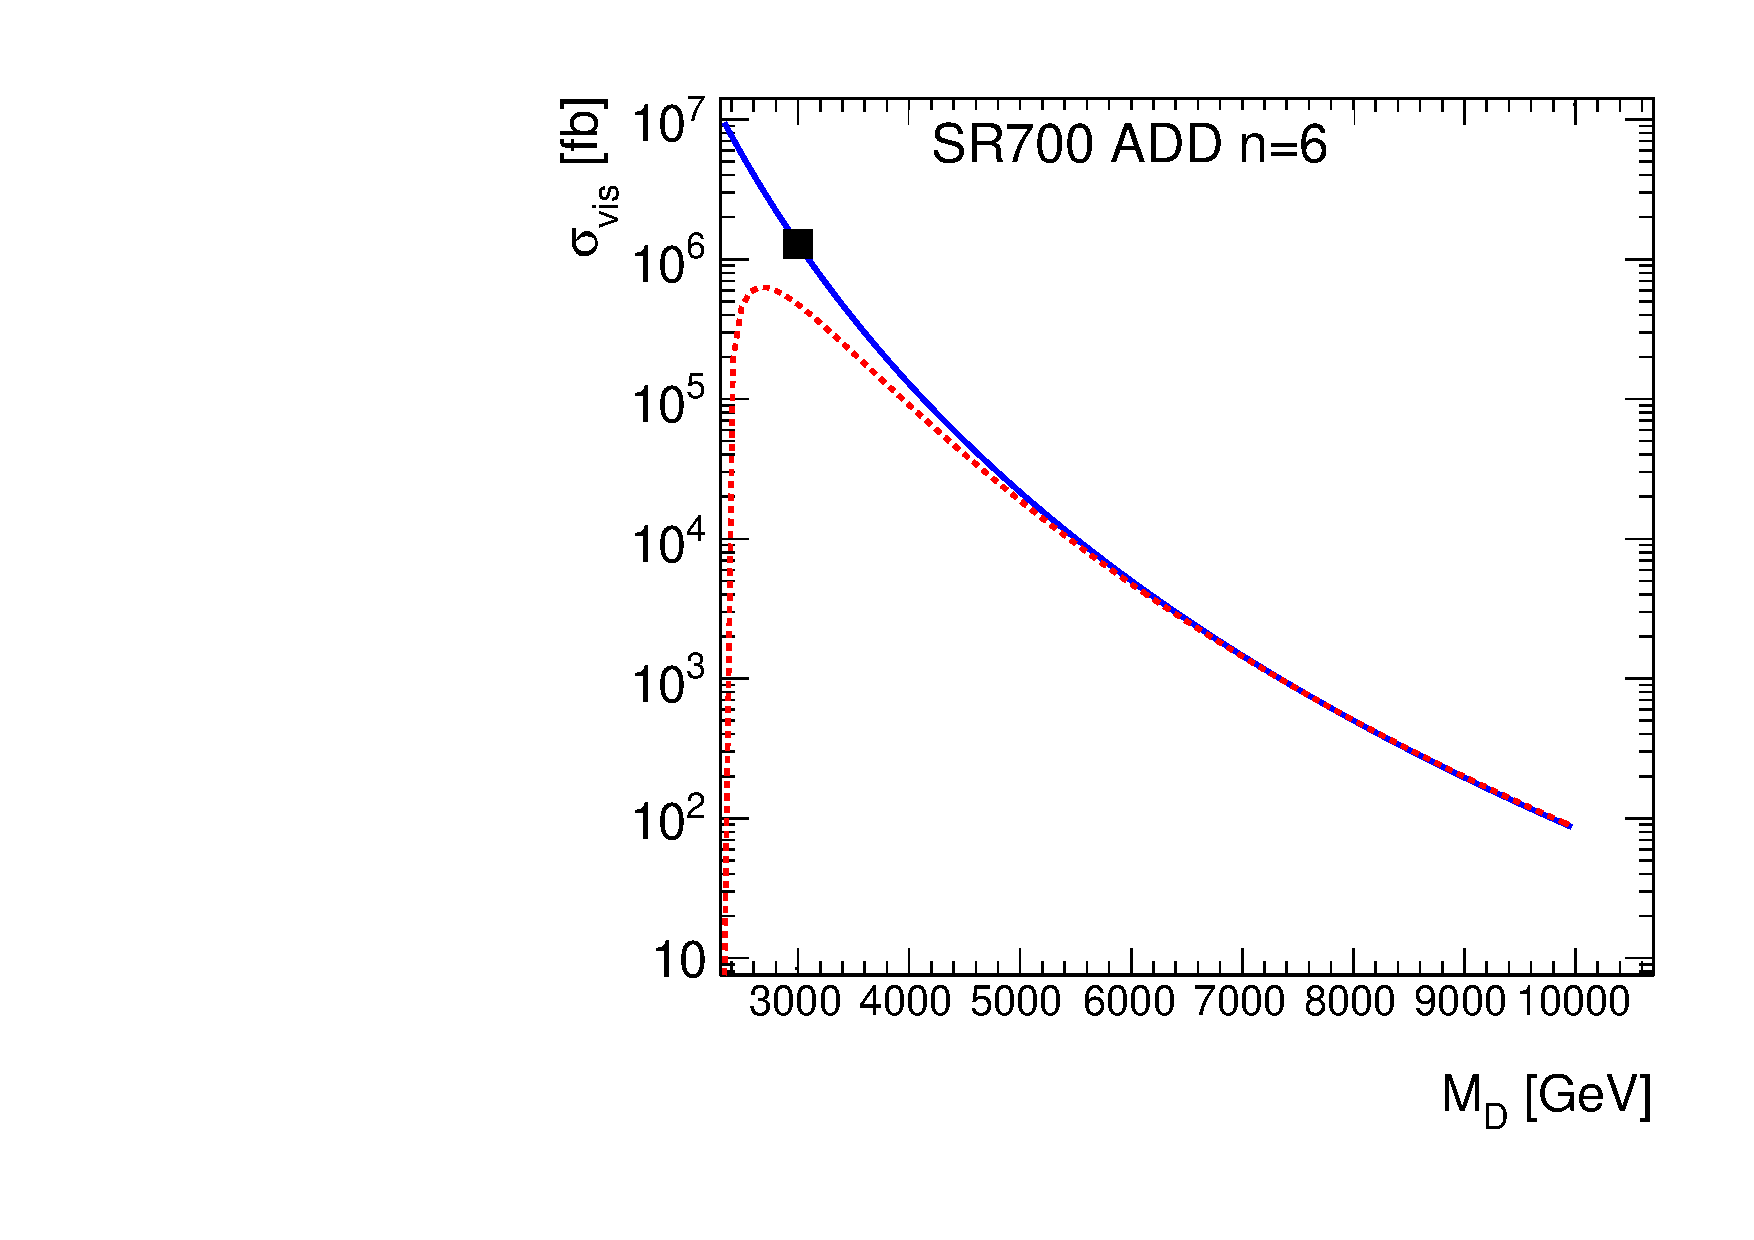
\includegraphics[width=\linewidth]{plot_sigma_visible_nD6_SR700}
    \caption{}
    \label{fig:sigma_vis_n6}
  \end{subfigure}
  \caption{Visible cross section as a function of $\md$ for the signal region
    where $250 < \met < 300$~GeV and $700 < \met < 800$~GeV for the ADD n = 3
    and 6 models. The solid line is the visible cross section when considering
    all events, while the dashed curve is built only from events where a
    $\md^4/\hat{s}^2$ weighting factor is applied for events where
    $\hat{s} > \md^2$. The black square is the nominal $\md$ value of the
    generated sample as listed in \cref{tab:sigma_md_ref}.}
  \label{fig:vis_sigma_trunc}
\end{figure}
%%% Local Variables:
%%% mode: latex
%%% TeX-master: "../search_for_DM_LED_with_ATLAS"
%%% End:
